\documentclass[11pt,a4paper,twoside]{report}

\usepackage[ngerman,USenglish]{babel} % Swap languages with \selectlanguage{...}
\usepackage[utf8]{inputenc} % to write characters (à,Ü,...) in the source
\usepackage[T1]{fontenc} % make characters (à,Ü,...) appear as such in the pdf
\usepackage{lmodern}
\usepackage{amsmath,amssymb,amsfonts} % math stuff
\usepackage{array} % better implementation of tabular and array environments
\usepackage{graphicx} % graphics inclusion
\usepackage{fancyhdr} % beautiful page headers/footers
\usepackage{emptypage} % removes header/footer from empty pages
\usepackage{microtype} % beautiful typesetting
\usepackage{verbatim} % typesetting raw text

% More packages.  Uncomment what you need:

% \usepackage{bbm} % if you need $\mathbbm{1}$
% \usepackage{mathrsfs} % if you need more math script fonts $\mathscr{A}$
% \usepackage{pifont} % more symbols, e.g., circled numbers

\usepackage{pict2e} % a better picture environment
\usepackage{tikz} % versatile drawing facilities
\usetikzlibrary{fit} % used for the example tikzpicture
\usepackage{pgfplots} % versatile plotting facilities

% \usepackage{psfrag}
% \usepackage[crop=pdfcrop,cleanup={.tex,.dvi,.ps,.pdf,.log,.aux,.idx,.toc,.out}]
% {pstool} % a pdf-compatible alternative to psfrag.

% \usepackage{amsthm} % or % \usepackage{theorem} % for theorems

% \usepackage{algorithmicx} % typesetting algorithms

% \usepackage[labelfont={md}]{subfig} % for sub-floats, e.g. sub-figures

\usepackage{url} % write URLs

% the last package to load:
\usepackage[bookmarksnumbered=true,hypertexnames=false]{hyperref} % hyperlinks

% Page layout
\setlength{\oddsidemargin}{2.5cm}
\setlength{\evensidemargin}{0.5cm}
\addtolength{\textheight}{0.0cm}
\addtolength{\textwidth}{0.0cm}
\addtolength{\topmargin}{0.0cm}
\setlength{\headheight}{3ex}

\renewcommand{\baselinestretch}{1.2}

% Here the document starts
\begin{document}

\pagenumbering{Roman}
\pagestyle{plain}

% Title page
\begin{titlepage}
  \begin{center}
    
\includegraphics[height=15mm]{gfx/ethlogo} \hfill
    
\includegraphics[height=15.5mm]{gfx/isilogo_left}
    \rule{\textwidth}{0.5pt}\\[1ex]
    {\Large Spring Semester 2014 \hfill 
      Prof.~H.-A.~Loeliger
    }

    \vspace{\stretch{5}}
    \LARGE Semester Thesis

    \vspace{\stretch{8}}
    \Huge\textbf{
      Phase-Locked Loops
    }
    
    \vspace{\stretch{10}}
    \LARGE{
      Daniel Gilgen\\
      and \\
      Fabio Marti \\
    }
    
    \vspace{\stretch{10}}
  \end{center}
  \rule{\textwidth}{0.5pt}\\[2ex]
  \noindent
  \begin{tabular}{@{}ll@{}}
    \Large Advisor: & \Large Nour Zalmai\\[1ex]
    \Large Co-Advisor: & \Large Lukas Bruderer
  \end{tabular}
\end{titlepage}

% Project description (optional)
\cleardoublepage
(Here the project description may be put in \ldots page 1)
\clearpage
(Here the project description may be put in \ldots page 2)
\cleardoublepage

% Dedication and/or quotation (optional)
\thispagestyle{empty}
\bigskip
\begin{center}   
  To Arwen
\end{center}

\vfill
\begin{quote}
  \itshape
  ``Among all the conundrums in the world, the Gordian knot is the most
  mysterious.''

  \hfill Anon.
\end{quote}
\vfill

\cleardoublepage

% Acknowledgments
\chapter*{Acknowledgements}
I would like to thank \ldots

(The chapter ``Acknowledments'' is better included by the command
\verb|\include{file}|.)

\vspace{11mm}
\noindent
Zürich, 00 March 2013

\vspace{19mm}
\noindent
Fabienne Fröhlich \hfill Mark Muster \hfill \null
\cleardoublepage

% English abstract
\thispagestyle{empty}
\begin{center} \huge \bfseries \abstractname \end{center}
Here comes the abstract \ldots

(The abstract is better included by the command \verb|\include{file}|.)
\clearpage

% Abstract in other language(s) (optional)
\thispagestyle{empty}
\begin{otherlanguage}{ngerman}
  \begin{center} \huge \bfseries \abstractname \end{center}
  Das ist die Zusammenfassung \ldots
  
  (Die Zusammenfassung sollte besser mittels des Befehls \verb|\include{file}|
  eingebunden werden.)
\end{otherlanguage}
\cleardoublepage

% Setup the fancy headers
\pagestyle{fancy}
\renewcommand{\chaptermark}[1]{\markboth{#1}{}}
\renewcommand{\sectionmark}[1]{\markright{\thesection\ #1}}
\fancyhead{}

% Table of contents
\fancyhead[LO]{\scshape \contentsname}
\fancyhead[RO]{\scshape Master's Thesis}
\fancyhead[LE]{\scshape Master's Thesis}
\fancyhead[RE]{\scshape \contentsname}
\pdfbookmark{\contentsname}{contentsbookmarkname}
\tableofcontents
\clearpage

% List of figures (optional)
\fancyhead[LO]{\scshape \listfigurename}
\fancyhead[RE]{\scshape \listfigurename}
\phantomsection\addcontentsline{toc}{chapter}{\numberline{}\listfigurename}
\listoffigures
\clearpage

% List of tables (optional)
\fancyhead[LO]{\scshape \listtablename}
\fancyhead[RE]{\scshape \listtablename}
\phantomsection\addcontentsline{toc}{chapter}{\numberline{}\listtablename}
\listoftables
\cleardoublepage

\setcounter{chapter}{0}
\setcounter{figure}{0}
\pagenumbering{arabic}
\fancyhead[LO]{\rightmark}
\fancyhead[RO]{\scshape \chaptername\ \thechapter}
\fancyhead[LE]{\scshape \chaptername\ \thechapter}
\fancyhead[RE]{\textsc{\leftmark}}

% Chapters
\chapter{Introduction}
(The chapters are better included by the command \verb|\include{file}|.)

This framework for your report hopefully helps you getting started quickly.  If
you are not familiar with \LaTeX{}, a good starting point is
\url{http://tobi.oetiker.ch/lshort/lshort.pdf}

\section{Compilation}
You can use shell commands to compile this document into a pdf file either as:
\begin{verbatim}
pdflatex report.tex
bibtex report
pdflatex report.tex
pdflatex report.tex
\end{verbatim}
or as:
\begin{verbatim}
latex report.tex
bibtex report
latex report.tex
latex report.tex
dvips report.dvi -o report.ps
ps2pdf report.ps
\end{verbatim}

Of course you can use this file with dedicated \LaTeX{} editors like Kile or
TexMaker, or you can call \texttt{(pdf)latex} from within a text editor that has
a \LaTeX{} mode, such as Emacs or Vim.

\section{Citations}

You can use \verb|bibtex| to include a citation, e.g. \cite{loeliger2007}.  For
every publication you would like to cite you have to add an entry in the
\verb|bibliograpy.bib| file.

\section{Math}
Different shapes $\phi$, $\Phi$, $\varPhi$, $x$, $\mathbf{x}$, $\boldsymbol{x}$,
$\boldsymbol{\phi}$, $\mathbb{R}$, $\mathcal{R}$, $\mathsf{E}$

An equation:
\begin{equation*}
  e = \lim_{k\to\infty} \left( 1 + \frac{1}{k} \right)^k
\end{equation*}

Aligned equations, this time with labels:
\begin{align}
  \label{eq:1}
  f(x) &= \sum_{k=1}^\infty \frac{1}{x^k}\\
  \label{eq:2}
  &= \log(1+e^x)
\end{align}
In Eq.~\eqref{eq:1} we have a sum.  In Eq.~\eqref{eq:2}, $e$ is Euler's number.

\section{Floats}
Floats are figures and tables that are allowed to appear anywhere on the page.

\subsection{Tables}
Table~\ref{tab:table} shows an example table.  Better spacing is achieved by
using either the \texttt{booktab} or the \texttt{mdwtab} package.

\begin{table}[htb]
  \centering
  \begin{tabular}{@{}lccp{5cm}@{}}
    \textbf{Fruit} & \multicolumn{2}{l}{\textbf{Some numbers}} & \textbf{An
      explanation}\\ \hline\hline
    Apple & 3 Pieces & 320 g & An apple a day keeps the doctor away.\\ \hline
    Pineapple & 2 Pieces & 540 g & Apples and pineapples share a part of their
    name. \\ \hline
    Strawberry & 1 Basket & 120 g & They do not continue to ripen after having
    been picked.\\ \hline 
  \end{tabular}
  \caption{An example table.}
  \label{tab:table}
\end{table}

\subsection{Figures}
Fig.~\ref{fig:pict} is drawn with the ordinary \LaTeX{} drawing commands.
Fig.~\ref{fig:tikz} is drawn with the Ti\emph{k}Z package.  Of course you can
also use your favorite stand-alone graphics drawing application to produce an
eps file (for \texttt{latex}) or a pdf file (for \texttt{pdflatex}) and include
this file, such as done in Fig.~\ref{fig:externalfig}.  Plotting can also be
done directly from a data file with the pgfplots package (which builds on the
Ti\emph{k}Z package) as exemplified in Fig.~\ref{fig:pgfplots}.

\begin{figure}[h]
  \centering
  \setlength{\unitlength}{1mm}
  \begin{picture}(39,21)
    \put(0,6){\vector(1,0){10}}
    \put(4,9){\makebox(0,0){$x(t)$}}
    \put(10,2){\framebox(8,8){$f(\cdot)$}}
    \put(18,6){\vector(1,0){5}}
    \put(26,6){\circle{6}}
    \put(26,6){\makebox(0,0){$+$}}
    \put(26,19){\vector(0,-1){10}}
    \put(25,15){\makebox(0,0)[r]{$z(t)$}}
    \put(29,6){\vector(1,0){10}}
    \put(35,9){\makebox(0,0){$y(t)$}}
    \multiput(8,0)(1.5,0){16}{\line(1,0){0.5}}
    \multiput(31,0)(0,1.5){14}{\line(0,1){0.5}}
    \multiput(8,0)(0,1.5){14}{\line(0,1){0.5}}
    \multiput(8,21)(1.5,0){16}{\line(1,0){0.5}}
  \end{picture}
  \caption{This is a figure drawn with the \texttt{picture} environment.}
  \label{fig:pict}
\end{figure}

\begin{figure}[htb]
  \centering
  \begin{tikzpicture}[>=latex,node distance=18mm,<-]
    \coordinate (x);
    \node[draw,right of=x] (f) {$f(\cdot)$} edge node[above] {$x(t)$} (x);
    \node[draw,circle,right of=f] (p) {$+$} edge (f);
    \coordinate[above of=p] (z) edge[->] node[left] {$z(t)$} (p);
    \coordinate[right of=p] edge node[above] {$y(t)$} (p);
    \node[draw,inner sep=2mm,dashed,fit=(f)(z)(p)] {};
  \end{tikzpicture}
  \caption{This is a figure drawn with the \texttt{tikzpicture} environment.}
  \label{fig:tikz}
\end{figure}

\begin{figure}[htb]
  \centering
  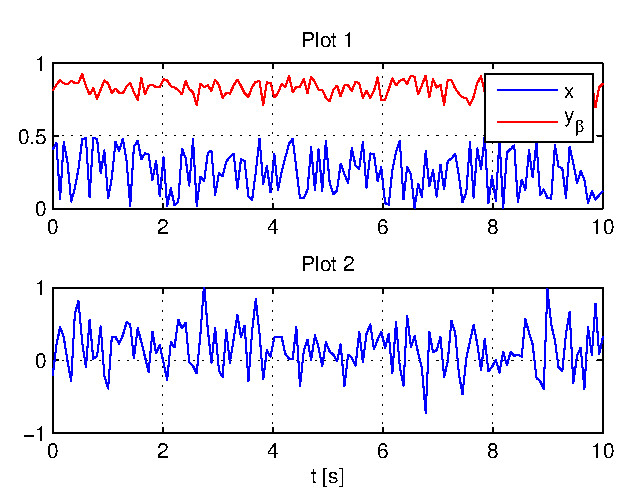
\includegraphics[width=\textwidth]{gfx/externalfig}
  \caption{A plot from an external eps or pdf file.}
  \label{fig:externalfig}
\end{figure}

\begin{figure}[htb]
  \centering
  \pgfplotstableread{data.dat}\plotdata
  \begin{tikzpicture}
    \begin{axis}[height=4.5cm,width=\textwidth,
      xmin=0,xmax=10,ymin=0,ymax=1,
      title=Plot 1]
      \addplot[blue] table[x index=0,y index=1] {\plotdata};
      \addplot[red] table[x index=0,y index=2] {\plotdata};
      \legend{$x$, $\gamma_\beta$}
    \end{axis}
    \begin{axis}[yshift=-4.5cm,height=4.5cm,width=\textwidth,
      xmin=0,xmax=10,ymin=-1,ymax=1,
      xlabel={$t\ [s]$},
      title=Plot 2]
      \addplot[blue] table[x index=0,y index=3] {\plotdata};
    \end{axis}
  \end{tikzpicture}
  \caption{A \texttt{pgfplots} plot.}
  \label{fig:pgfplots}
\end{figure}

\clearpage

% Appendices (optional)
\appendix
\fancyhead[LO]{\rightmark}
\fancyhead[RO]{\scshape\appendixname\ \thechapter}
\fancyhead[LE]{\scshape\appendixname\ \thechapter}
\fancyhead[RE]{\textsc{\leftmark}}

\chapter[Proof of Upper Bound]{Proof for the Lower Bound on the Number of
  Conundrums}
Since we classify the Gordian knot as a conundrum, there is at least one such.

\clearpage

% Bibliography
\fancyhead[LO]{\scshape\bibname}
\fancyhead[RO]{\scshape\appendixname}
\fancyhead[LE]{\scshape\appendixname}
\fancyhead[RE]{\scshape\bibname}

\bibliographystyle{unsrt} % bibliography style in order of first citation

\phantomsection\addcontentsline{toc}{chapter}{\numberline{}\bibname}
\bibliography{IEEEabrv,bibliography}

\end{document}
